\documentclass{beamer}

%\usetheme{Madrid}
\setbeameroption{show notes}
\setbeamertemplate{navigation symbols}{}

\usepackage{listings}
\lstset{language=[ISO]C++,
        basicstyle=\ttfamily\scriptsize,
        keywordstyle=\color{blue},
        stringstyle=\color{red},
        commentstyle=\color{green},
        frame=single,
        }
        
\usepackage{lmodern}
\usepackage{color}

\title{Advanced Programming Techniques}
\author{David Schneider}


\begin{document}

\frame{\titlepage}

\part{Overview}

%%%%%%%%%%%%%%%%%%%%%%%%%%%%%%%%%%%%%%%%%%%%%%%%%%%%%%%%%%%%%%%%%%%%%
\begin{frame}
\begin{description}
\item[Umfang] 5 ECTS
\item[Lehr- und Lernformen]: Vorlesung mit integrierter Übung
\item[Prüfungsmodalitäten]: LV-abschließende Prüfung; Projektarbeit - Prüfungsgespräch über die Projektarbeit
\end{description}
\end{frame}

%%%%%%%%%%%%%%%%%%%%%%%%%%%%%%%%%%%%%%%%%%%%%%%%%%%%%%%%%%%%%%%%%%%%%
\begin{frame}{Lehrinhalte}
Erlernen von Konzepten der objektorientierten Programmierung anhand der
Programmiersprache C++ (Klassen und Objekte, Kapselung, Vererbung und
Polymorphismus), Fehler- und Ausnahmebehandlung, Coding Guidelines, Design
Patterns, Design for Testability. Bildung von Modellen, Abstraktion,
Lösungsfindung und Evaluation in der  objektorientierten Programmierung.
Einbindung vorhandener Lösungskonzepte und systematische Herangehensweise an
konkreten Problemstellungen.
\end{frame}

%%%%%%%%%%%%%%%%%%%%%%%%%%%%%%%%%%%%%%%%%%%%%%%%%%%%%%%%%%%%%%%%%%%%%
\begin{frame}{Literaturempfehlungen}
\begin{itemize}
\item E. Gamma et al., Design Patterns, Addison-Wesley (1995)
\item R. Martin, Clean Code, Prentice Hall Pearson Education (2009)
\item B. Stroustrup: The C++ Programming Language, 4th edition, Addison Wesley
(2013)
\item A. Alexandrescu: Modern C++ Design, Addison Wesley (2001)
\item H. Sutter: C++ Coding Standards, Addison Wesley (2004)
\end{itemize}
\end{frame}

\begin{frame}{Termine 2016}
\begin{table}
\begin{tabular}{l | l }
Datum & Raum \\
\hline
23.09.2016 & EDV5 \\
30.09.2016 & EDV2 \\
07.10.2016 & EDV2 \\
14.10.2016 & EDV2 \\
21.10.2016 & EDV2 \\
28.10.2016 & EDV2 \\
04.11.2016 & EDV2 \\
11.11.2016 & EDV2 \\
18.11.2016 & EDV2 \\
25.11.2016 & EDV2
\end{tabular}
\end{table}
\end{frame}

\part{Introduction}

\section{Introduction}

\subsection{Object-oriented programming}

\begin{frame}{Pradigma}
OOP is a programming pradigma

Objects contain
\begin{itemize}
\item data (ak. attribute)
\item code (ak. methods)
\end{itemize}

\end{frame}

\begin{frame}{OOP vs. Procedural}

\begin{block}{Procedural}
data tends to be highly decoupled from the functions that operate on it
\end{block}

\begin{block}{Object-oriented}
data tends to carry with it a collection of functions
\end{block}

\note{http://stackoverflow.com/a/552474/6632389}

\end{frame}

\subsection{Object-oriented concepts}

\begin{frame}{Classes and objects}

\begin{block}{Class}
The blueprint for an object. Defines how a object should be created.
\end{block}

\begin{block}{Object}
An instance of a class. Gets created during runtime.
\end{block}

\end{frame}

\begin{frame}{Information hidding}
Encapsulate data and hide the internal structure from caller. This allows
changing the internal details without affecting 
\end{frame}

\begin{frame}{Inheritance}
Exentend or overwrite functionality of another class.
\end{frame}

\begin{frame}{Interface}
Define a method without implementing it as an interface to be used by other
classes.
\end{frame}

\begin{frame}{Polymorphism}
\framesubtitle{aka Subtyping}
Define a implementation for a specialized type.
\end{frame}

\subsection{C++}
\begin{frame}{C++ - Overview}
\begin{itemize}
  \item compiled language
  \item general-purpose programming language
  \item Multi-pradigma
  \begin{itemize}
    \item procedural
    \item functional
    \item object-oriented
    \item generic
  \end{itemize}
  \item statically typed
  \item allows low-level memory manipulation
  \item designed for large, resource constrained systems 
\end{itemize}
\end{frame}


\begin{frame}{C++ - Standardization}
\itemize{}
\item[1979] C with Classes first implemented 
\item[1998] C++98 (ISO/IEC 14882:1998) 
\item[2003] C++03 (ISO/IEC 14882:2003)
\item[2011] C++11 (ISO/IEC 14882:2011)
\note[item]{C++11 major extension over C++03} 
\item[2014] C++14 (ISO/IEC 14882:2014)
\note[item]{C++14 small extension over C++11, featuring mainly bug fixes
 and small improvements}
\item[2017] C++17 (also called C++1z)
\end{frame}

\begin{frame}{Emedded Systems}
\begin{itemize}
  \item Embedded C++ (still in use?)
\end{itemize}
\end{frame}

\part{Buildsystem}

\section{Buildsystem}
\subsection{Tools}
\begin{frame}{Tools}
\begin{description}
  \item[Code:Blocks] \url{http://www.codeblocks.org/}
  \note[item]{Code:Blocks: IDE, Contains GCC compiler}
  \item[Git for Windows] \url{https://git-for-windows.github.io/}
  \note[item]{Git for Windows: Git CLI (git.exe) used as back-end for
  TortoiseGit}
  \item[TortoiseGit] \url{https://tortoisegit.org/}
  \item[CMake] \url{https://cmake.org/}  
\end{description}

\end{frame}

\part{OO-Basics}

\section{OO-Basics}

\begin{frame}
Design is all about changable code.
Code is written once, but read many times.
\end{frame}

\subsection{Features}

\begin{frame}
accessibility
\end{frame}

\begin{frame}{Encapsulation}
abstraction
information hidding
hide internal details, which allows changing this details
\end{frame}

\begin{frame}{Inheritance}
Base class
Abstract class
\end{frame}

\begin{frame}{Composition and delegation}
TODO
\end{frame}

\begin{frame}{Polymorphism}
subtyping
\end{frame}

\begin{frame}{Open recursion}
Virtual methods

\lstinputlisting[caption=Open recursion]{lst/open_recursion.cpp}


\end{frame}


\subsection{Pattern}


\frame{GRASP}

\subsection{SOLID}

\begin{frame}{S.O.L.I.D - Principals}
Defined by Robert C. Martin (Oncle Bob)


\begin{description}
\item [S] Single-responsiblity principle
\item [O] Open-closed principle
\item [L] Liskov substitution principle
\item [I] Interface segregation principle
\item [D] Dependency Inversion Principle
\end{description}
\end{frame}

\begin{frame}{Single-responsiblity principle}
a class should have only a single responsibility (i.e. only one potential change
in the software's specification should be able to affect the specification of the class)
\end{frame}

\begin{frame}{Open-closed principle}
''A module should be open for extension but closed for modification''
\end{frame}

\begin{frame}{Liskov substitution principle}
''objects in a program should be replaceable with instances of their subtypes
without altering the correctness of that program.''
\end{frame}

\begin{frame}{Interface segregation principle}
\end{frame}

\begin{frame}{Dependency Inversion Principle}
\end{frame}

\subsection{Clean Code}

\part{Object Oriented Design - Pattern}
\section{Object Oriented Design - Pattern}

\begin{frame}{Pattern}
\begin{itemize}
  \item singelton
  \item factory
  \item command
  \item observer
  \item strategy
  \item visitor
  \item null object
  \item adapter
  \item proxy
  \item fly-weight
\end{itemize}
\end{frame}

\part{C++ Tutorial}{cpp-tutorial}

\begin{frame}{Source}
C++ Language Tutorial
Source: \url{http://www.cplusplus.com/doc/tutorial/}
\note{reference on cplusplus.com contains some errors,
http://stackoverflow.com/questions/6520052/whats-wrong-with-cplusplus-com}
\end{frame}

\section{Basics of C++}

\subsection{Structure of a program}
\begin{frame}

\end{frame}

\subsection{Variables and types}
\begin{frame}

\end{frame}


%%%%%%%%%%%%%%%%%%%%%%%%%%%%%%%%%%%%%%%%%%%%%%%%%%%%%%%%%%%%%%%%%%%%%
\begin{frame}[fragile]{Identifiers}
\begin{itemize}
  \item case-sensitive
  \item sequence of one or more letters, digits, or underscore
  \item always begin with a letter
  \item begin with underscore allowd, but used for special cases
  \item many reserved keywords, which can't be used as identifiers 
\end{itemize}
\begin{lstlisting}[caption=Identifiers Examples]
aNumber
my1st_variable
SomeMoreIdentifier
\end{lstlisting}
\end{frame}

%%%%%%%%%%%%%%%%%%%%%%%%%%%%%%%%%%%%%%%%%%%%%%%%%%%%%%%%%%%%%%%%%%%%%
\begin{frame}{Fundamental data types}
\begin{itemize}
  \item Character types
  \item Numerical integer types
  \item Floating-point types
  \item Boolean type
\end{itemize}
\end{frame}

%%%%%%%%%%%%%%%%%%%%%%%%%%%%%%%%%%%%%%%%%%%%%%%%%%%%%%%%%%%%%%%%%%%%%
\begin{frame}{Fundamental data types}
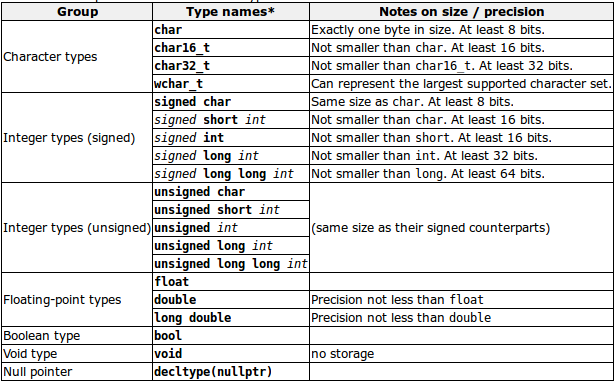
\includegraphics[scale=0.48]{img/FundamentalTypes.png}
\end{frame}

%%%%%%%%%%%%%%%%%%%%%%%%%%%%%%%%%%%%%%%%%%%%%%%%%%%%%%%%%%%%%%%%%%%%%
\begin{frame}[fragile]{Declaration of variables}
\begin{itemize}
  \item Strongly typed
  \item Every variable to be declared before first use
\end{itemize}
\begin{lstlisting}[caption=Variable declaration]
int aNumber;
float aFloatingPointerNumber;
\end{lstlisting}
\end{frame}

%%%%%%%%%%%%%%%%%%%%%%%%%%%%%%%%%%%%%%%%%%%%%%%%%%%%%%%%%%%%%%%%%%%%%
\begin{frame}[fragile]{Initialization of variables}
\begin{definition}{Initialization}
   Set the value of variable during declaration. 
\end{definition}
\begin{lstlisting}[caption=Variable initialization]
int aNumber = 5;
float aFloatingPointerNumber(6);
\end{lstlisting}
\end{frame}

%%%%%%%%%%%%%%%%%%%%%%%%%%%%%%%%%%%%%%%%%%%%%%%%%%%%%%%%%%%%%%%%%%%%%
\begin{frame}[fragile]{Type deduction: auto and decltype}
Automatic type determination with keyword `auto`.

Usefull for cases where the explicitly type is not so importent or the type is
so complex (ex. with templates) that it's hard the define the type correct.

\lstinputlisting[caption=Auto Type]{lst/AutoType.cpp}

\end{frame}

%%%%%%%%%%%%%%%%%%%%%%%%%%%%%%%%%%%%%%%%%%%%%%%%%%%%%%%%%%%%%%%%%%%%%
\begin{frame}{Introduction to strings}
Example for compound types: std::string

\lstinputlisting[caption=String Example]{lst/SimpleString.cpp}

\end{frame}


\subsection{Constants}

%%%%%%%%%%%%%%%%%%%%%%%%%%%%%%%%%%%%%%%%%%%%%%%%%%%%%%%%%%%%%%%%%%%%%
\begin{frame}[fragile]{Literals}

\begin{lstlisting}[caption=Integer Numerals]
75         // decimal
0113       // octal
0x4b       // hexadecimal
\end{lstlisting}

\end{frame}

%%%%%%%%%%%%%%%%%%%%%%%%%%%%%%%%%%%%%%%%%%%%%%%%%%%%%%%%%%%%%%%%%%%%%
\begin{frame}[fragile]{Literals}

\begin{lstlisting}[caption=Floating Point Numerals]
3.14159    // 3.14159
6.02e23    // 6.02 x 10^23
1.6e-19    // 1.6 x 10^-19
3.0        // 3.0
\end{lstlisting}

\end{frame}

%%%%%%%%%%%%%%%%%%%%%%%%%%%%%%%%%%%%%%%%%%%%%%%%%%%%%%%%%%%%%%%%%%%%%
\begin{frame}{Literals}
\begin{table}
\begin{tabular}{l | c}
Suffix & Type modifier \\
\hline
u or U & unsigned \\
l or L & long \\
ll or LL & long long \\
f or F & float \\
l or L & long double
\end{tabular}
\caption{Type modifier}
\end{table}

\end{frame}

%%%%%%%%%%%%%%%%%%%%%%%%%%%%%%%%%%%%%%%%%%%%%%%%%%%%%%%%%%%%%%%%%%%%%
\begin{frame}[fragile]{Character and string literals}
\begin{description}
\item[Character] A singel character, between single quotes
\item[String] Null-terminated string, between double quotes 
\end{description}
\begin{lstlisting}[caption=Character and string literals]
'z'
'p'
"Hello world"
"How do you do?"
\end{lstlisting}

\end{frame}

%%%%%%%%%%%%%%%%%%%%%%%%%%%%%%%%%%%%%%%%%%%%%%%%%%%%%%%%%%%%%%%%%%%%%
\begin{frame}[fragile]{Other literals}
\begin{description}
\item[Boolean] true and false
\item[Null-Pointer] reserved value to indicated, that a pointer doesn't refer to
a valid object
\end{description}
\begin{lstlisting}[caption=Other literals]
bool foo = true;
bool bar = false;
int* p = nullptr;
\end{lstlisting}
\end{frame}


%%%%%%%%%%%%%%%%%%%%%%%%%%%%%%%%%%%%%%%%%%%%%%%%%%%%%%%%%%%%%%%%%%%%%
\begin{frame}[fragile]{Typed constant expressions}
\begin{lstlisting}[caption=Typed constant expressions]
const double pi = 3.1415926;
const char tab = '\t';
\end{lstlisting}
\end{frame}

%%%%%%%%%%%%%%%%%%%%%%%%%%%%%%%%%%%%%%%%%%%%%%%%%%%%%%%%%%%%%%%%%%%%%
\begin{frame}[fragile]{Preprocessor definitions}
\begin{lstlisting}[caption=Preprocessor definitions]
#define PI 3.14159
#define NEWLINE '\n'
\end{lstlisting}

\end{frame}


\subsection{Operators}
\subsection{Basic Input/Output}

\section{Program structure}
\subsection{Control Structures}
\begin{frame}

\end{frame}

\subsection{Functions}
\begin{frame}

\end{frame}

\subsection{Overloads and templates}
\begin{frame}

\end{frame}
\subsection{Name visibility}
\begin{frame}

\end{frame}

\section{Compound data types}
\subsection{Arrays}
\begin{frame}

\end{frame}

\subsection{Character sequences}
\begin{frame}

\end{frame}

\subsection{Pointers}
\begin{frame}

\end{frame}

\subsection{Dynamic Memory}
\begin{frame}

\end{frame}

\subsection{Data structures}
\begin{frame}

\end{frame}

\subsection{Other data types}
\begin{frame}

\end{frame}


\section{Classes}
\subsection{Classes}
\begin{frame}

\end{frame}

\subsection{Special members}
\begin{frame}

\end{frame}

\subsection{Friendship and inheritance}
\begin{frame}

\end{frame}

\subsection{Polymorphism}
\begin{frame}

\end{frame}


\section{Other language features}
\subsection{Type conversions}
\begin{frame}

\end{frame}

\subsection{Exceptions}
\begin{frame}

\end{frame}

\subsection{Preprocessor directives}
\begin{frame}

\end{frame}


\part{C++ and C}
\section{C++ and C}
\begin{frame}

\end{frame}

\part{Standards}
\section{Standards}
\begin{frame}

\end{frame}


\part{Clean Code}
\section{Clean Code}
\begin{frame}

\end{frame}


\part{Coding Standards}
\section{MISRA}
\begin{frame}

\end{frame}


\part{Testing}
\section{TODO}
\subsection{Test-pyramid}
\begin{frame}

\end{frame}

\subsection{Unittest (SIL-test)}
\begin{frame}

\end{frame}

\subsection{Design for testability}
\begin{frame}

\end{frame}

\subsubsection{test}
\begin{frame}

\end{frame}


\end{document}
